\documentclass[a4paper]{article}

\usepackage[english]{babel}
\usepackage[utf8]{inputenc}
\usepackage{amsmath,amssymb, amsthm}
\usepackage{graphicx}
\usepackage{amssymb}
\usepackage{verbatim}
\usepackage{gensymb}
\usepackage{bm}

% \usepackage{draftwatermark}
% \SetWatermarkText{DRAFT}
% \SetWatermarkScale{3}

\usepackage[colorinlistoftodos]{todonotes}
\usetikzlibrary{positioning,arrows}

\theoremstyle{plain}

\theoremstyle{definition}



\newcommand{\thering}
{
\mathcal{O}_{-D}
}

\newcommand{\thefield}
{
\mathbb{Q}(\sqrt{-D})
}

\newcommand{\M}
{
\mathcal{M}
}

\newcommand{\norm}[1]
{
\left[ #1 \right]
}

\newcommand{\conj}[1]
{
\overline{#1}
}

\newcommand{\trans}[1]
{
\textbf{T}(#1)
}

\newcommand{\ideal}[1]
{
\left\langle #1 \right\rangle
}

\newcommand{\conjid}[1]
{
\overline{#1}
}

\newcommand{\id}[1]
{
{#1}
}

\newtheorem*{lem1}{Lemma 1}
\newtheorem*{lem2}{Lemma 2}
\newtheorem*{thm1}{Theorem}
\newtheorem*{cor1}{Corollary 1}
\newtheorem*{cor2}{Corollary 2}
\newtheorem*{prop1}{Proposition}


\begin{document}
\begin{center}
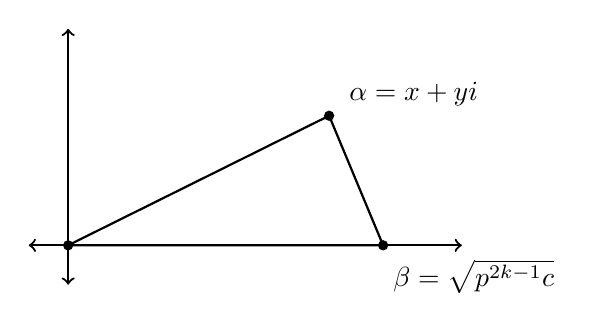
\begin{tikzpicture}[thick,scale=1.0, every node/.style={scale=1.0}]
  
%%%%%%%%%%%%%%%%%%%%%%%%%%%%%%%%%%%%%%%%%%%%%%%
%%%%%%%%%%%%%%%%%  Figure 1 %%%%%%%%%%%%%%%%%%%
%%%%%%%%%%%%%%%%%%%%%%%%%%%%%%%%%%%%%%%%%%%%%%%

  % Draw axes
  \draw[thick,<->] (-0.5,0) -- (5,0);
  \draw[thick,<->] (0,-0.5) -- (0,2.75);
  
  
  % Draw triangle
  \draw[thick] (0,0) -- (35*.1142857,0) -- (29*.1142857,14.4*.1142857) -- (0,0);
  
  % Plot and label vertices
  	% Origin
  \draw[fill] (0,0) circle (.5mm);
  
  	% Right vertex
  \draw[fill] (35*.1142857,0) circle (.5mm);
  \draw (35*.1142857,-.05) node[below right] {$\beta = \sqrt{p^{2k-1}c}$};
  
  	% Top vertex
  \draw[fill] (29*.1142857,14.4*.1142857) circle (.5mm);
  \draw (30.1*.1142857,14.4*.1142857) node[above right] {$\alpha = x + yi$};
   

\end{tikzpicture}
\end{center}
\begin{lem1}

Let $\M$ be a primitive integer norm pointset with characteristic $D$.  If $p$ is a rational prime that is also prime in $\thering$, and $p$ divides the norm of some pairwise difference in $\M$, then $p$ divides it with even multiplicity.

\end{lem1}

\begin{proof}

Translate and possibly reflect $\M$ in the plane so that, of the two points whose pairwise distance's norm $p$ divides, one lies at the origin and the other lies on the positive $x$-axis.  Denote the latter point by $\beta$.

We will assume, for an contradiction, that $p$ divides $\norm{\beta}$ with odd multiplicity - that is, there exist some positive integers $c$ and $k$ such that $\beta = \sqrt{p^{2k-1}c}$, but $p$ does not divide $c$.

Now let $\alpha$ be any other arbitrary point in $\M$.  We will show that $\alpha$ takes the form 
\begin{align}
\alpha = \frac{\delta\sqrt{p}}{2\sqrt{c}}
\end{align}
for some $\delta \in \thering$.

Since $\norm{\alpha}, \norm{\beta}$, and $\norm{\alpha - \beta}$ are all integers, we know that
$$\norm{\alpha} - \norm{\beta} - \norm{\alpha - \beta} = \alpha\conj{\beta} + \conj{\alpha}\beta = 2x\sqrt{p^{2k-1}c} = a$$ for some $a \in \mathbb{Z}$ such that $x = \dfrac{a}{2\sqrt{p^{2k-1}c}}$.

The area of the triangle formed by $0$, $\alpha$, and $\beta$ is $$\frac{1}{2}y\sqrt{p^{2k-1}c} = \frac{b}{4}\sqrt{D}$$ for some $b \in \mathbb{Z}$ such that $y = \dfrac{b\sqrt{D}}{2\sqrt{p^{2k-1}c}}$.

Now, letting $\gamma = a + b\sqrt{-D} \in \thering$, we obtain the following expression for $\alpha$:

$$\alpha = x + y\sqrt{-D} = \frac{a + b\sqrt{-D}}{2\sqrt{p^{2k-1}c}} = \frac{\gamma}{2\sqrt{p^{2k-1}c}}.$$

Since $\alpha$ has integer norm, the norm of its denominator must divide the norm of $\gamma$.  So $p^{2k-1} \mid \gamma \conj{\gamma}$.  Since $p$ is prime in $\thering$, we must have either $p^k \mid \gamma$ or $p^k \mid \conj{\gamma}$.  Since $p$ is rational, either case implies that $p^k \mid \gamma$.  Thus there exists some $\delta \in \thering$ such that $\gamma = p^k\delta$, hence proving $\alpha$ takes the form given in (1).

First, assume that $p \neq 2$.  Since $p \nmid c$, we must have $2c \mid \norm{\delta}$, thus $p \mid \norm{\alpha}$.  Now, instead assume $p = 2$.  Then $\alpha = \dfrac{\delta}{\sqrt{2c}}$, so $2 \mid \delta \conj{\delta}$, hence $2 \mid \delta$ since we have assumed $p = 2$ is prime.  So $\alpha = \dfrac{\delta'\sqrt{p}}{\sqrt{c}}$ for some $\delta' \in \thering$, and again $p \mid \norm{\alpha}$.

Since  $$\norm{\alpha - \beta} = \norm{\alpha} + \norm{\beta} - \alpha\conj{\beta} - \conj{\alpha}\beta = \norm{\alpha} + \norm{\beta} - \sqrt{p^{2k-1}c} \left(\frac{\delta\sqrt{p}}{2\sqrt{c}} + \conj{\frac{\delta\sqrt{p}}{2\sqrt{c}}} \right)$$ $$ = \norm{\alpha} + \norm{\beta} - p^kRe(\delta).$$  Since $p$ divides all three of these terms, it divides $\norm{\alpha - \beta}$.

Now, since $\alpha$ was an arbitrary point in $\M$ other than $0$ or $\beta$, we know if we take some other point $\eta \in \M$, $p$ will divide both $\norm{\eta}$ and $\norm{\eta - \beta}$.  It will also be of the form $\eta = \dfrac{\varepsilon\sqrt{p}}{2\sqrt{c}}$ given in (1), thus $$ p \mid p\frac{\norm{\delta - \varepsilon}}{4c} = \norm{\alpha - \eta}$$ since $p \nmid c$ and, again, if $p = 2$ then $p$ divides both $\delta$ and $\varepsilon$.  Therefore, $p$ divides the norms of all pairwise differences in $\M$, contradicting our assumption that $\M$ is primitive.



\end{proof}


\begin{lem2}

Let $\M$ be an integer norm pointset with characteristic $D$, and let $s$ be the greatest common divisor of the norms of all pairwise distances in $M$.  The following are equivalent:
\begin{enumerate}
\item For every $\alpha \in \M$ there exists an ideal $L \subset \thering$, not necessarily unique, such that $\ideal{\norm{\alpha}} = L \conjid{L}$
\item Every prime $p$ which is also prime in $\thering$ divides $s$ with even multiplicity.  In particular, this occurs if $\M$ is primitive.
\end{enumerate}
\end{lem2}

\begin{proof}
Scale $\M$ down by $\sqrt{s}$ to obtain a primitive integer pointset, and let $\alpha \in \M$.  By Lemma 1, every rational prime $p$ which is also prime in $\thering$ divides $\frac{\norm{\alpha}}{s}$ with even multiplicity, so factoring $\ideal{\norm{\alpha}}$ into prime ideals gives

\begin{align*}
\ideal{\frac{\norm{\alpha}}{s}} &= \ideal{p_1}^{2k_1} \cdots \ideal{p_k}^{2k_m} L_1 \conjid{L_1} \cdots L_n \conjid{L_n}
\\
&= \left(\ideal{p_1}^{k_1} \cdots \ideal{p_k}^{k_m} L_1 \cdots L_n \right)  \left( \ideal{p_1}^{k_1} \cdots \ideal{p_k}^{k_m} \conjid{L_1} \cdots \conjid{L_n} \right)
\\
&= J \conjid{J}
\end{align*}

where $J = \ideal{p_1}^{k_1} \cdots \ideal{p_k}^{k_m} L_1 \cdots L_n$.  Similarly, factoring $s$ into prime ideals gives
$$\ideal{\norm{\alpha}} = \ideal{s}\ideal{\frac{\norm{\alpha}}{s}} = \ideal{q_1}^{j_1} \cdots \ideal{q_k}^{j_m} H_1 \conjid{H_1} \cdots H_n \conjid{H_n}J\conjid{J}.$$  This factorization becomes $L \conjid{L}$ for some ideal $L$ if and only if each $j_i$ is even.

\end{proof}

\begin{thm1}
$\thering$ contains an element of norm $\norm{\alpha}$ if and only if $\ideal{\norm{\alpha}}$ has such a factorization where $L$ is principal for some $\alpha \in \M$.
\end{thm1}

\begin{proof}
Suppose assume the norm of some $\alpha \in \M$ has such a factorization where $L$ is principal, and let $\beta$ be a generator of $L$.  Then $\norm{\beta} = \norm{\alpha}$.

For the other direction, assume $\beta$ has norm $\norm{\alpha}$.  Then $\norm{\ideal{\alpha}} = \ideal{\beta}\ideal{\conjid{\beta}}$ gives such a factorization where $L$ is principal.


\end{proof}

\noindent Little Corollary: If for some $\alpha \in \M$ no such factorization exists where $L$ is principal, then clearly $\M$ does not embed in $\thering$.

\begin{cor1}

Suppose an integer norm pointset $\M$ has characteristic $D$, where $D$ is a Heegner number, and let $s$ be the greatest common divisor of the norms of all pairwise distances in $\M$.
$\M$ embeds in $\thering$ if and only if every prime $p$ which is also prime in $\thering$ divides $s$ with even multiplicity.
\\
\indent In particular, every primitive integer norm pointset with characteristic $D$ embeds in $\thering$.

\end{cor1}

\begin{proof}
If some prime $p$ which is also prime in $\thering$ does not divide $s$ with even multiplicity, then no such factorization exists.  So for every $\alpha \in \M$, $\thering$ contains no element of norm $\norm{\alpha}$, thus $\M$ cannot embed in $\thering$.

Now suppose every prime $p$ which is also prime in $\thering$ does divide $s$ with even multiplicity.  Then the norm of some $\alpha \in \M$ has such a factorization, and since $\thering$ is a principal ideal domain, $L$ is principal.  So there exists an element of norm $\norm{\alpha}$ for some $\alpha \in \M$.  Thus $\M$ embeds in $\thefield$.  Since the square of every ideal of $\thering$ is principal, $\M$ embeds in $\thering$.

\end{proof}


\end{document}
